% =============================================================================
%  ADAPT-Rehab -- Figure 1: System Architecture Overview (Standalone)
%  Based on 5-stage horizontal Mermaid diagram with detailed parameters.
%  Compile: pdflatex fig1_architecture.tex
%  Color palette: draw.io two-accent (Blue #1F4E79 + Red #C0392B + neutrals)
% =============================================================================
\documentclass[tikz,border=8pt]{standalone}
\usepackage[T1]{fontenc}
\usepackage[scaled]{helvet}
\renewcommand{\familydefault}{\sfdefault}
\usetikzlibrary{positioning,arrows.meta,calc,fit,backgrounds,shapes.misc}

% --- draw.io Color Palette (Two-Accent: Blue + Red + Neutrals) ----------------
\definecolor{AccentBlue}{HTML}{1F4E79}
\definecolor{AccentBlueFill}{HTML}{D9E2F3}
\definecolor{AccentRed}{HTML}{C0392B}
\definecolor{AccentRedFill}{HTML}{FADBD8}
\definecolor{OutputGreen}{HTML}{27AE60}
\definecolor{OutputGreenFill}{HTML}{EAFAF1}
\definecolor{NeutralBorder}{HTML}{2C3E50}
\definecolor{NeutralColFill}{HTML}{F4F6F7}
\definecolor{NeutralMid}{HTML}{566573}
\definecolor{TextMain}{HTML}{1B2631}
\definecolor{TextSub}{HTML}{566573}
\definecolor{White}{HTML}{FFFFFF}

% --- Layout Constants (cm) ----------------------------------------------------
\newcommand{\colW}{3.5}
\newcommand{\colH}{8.2}
\newcommand{\colGap}{0.55}
\newcommand{\boxW}{3.1}
\newcommand{\boxH}{0.95}
\newcommand{\titleH}{0.6}

% --- Component Box Helper Macro ----------------------------------------------
% #1: x-center, #2: y-center, #3: title (bold), #4: subtitle (italic)
\newcommand{\compbox}[4]{%
  \node[rounded corners=4pt, draw=NeutralBorder, line width=1.1pt,
        fill=White, minimum width=\boxW cm, minimum height=\boxH cm,
        align=center, text=TextMain] (tmp) at (#1,#2) {};
  \node[align=center, text=TextMain, font=\bfseries\footnotesize, inner sep=1pt]
        at ($(tmp.north)+(0,-0.28)$) {#3};
  \node[align=center, text=TextSub, font=\scriptsize\itshape, inner sep=1pt]
        at ($(tmp.south)+(0,0.28)$) {#4};
}

% --- Highlighted Box (blue accent border) -------------------------------------
\newcommand{\hlbox}[4]{%
  \node[rounded corners=4pt, draw=AccentBlue, line width=1.5pt,
        fill=White, minimum width=\boxW cm, minimum height=\boxH cm,
        align=center, text=TextMain] (tmp) at (#1,#2) {};
  \node[align=center, text=TextMain, font=\bfseries\footnotesize, inner sep=1pt]
        at ($(tmp.north)+(0,-0.28)$) {#3};
  \node[align=center, text=TextSub, font=\scriptsize\itshape, inner sep=1pt]
        at ($(tmp.south)+(0,0.28)$) {#4};
}

% --- Red-accent Box -----------------------------------------------------------
\newcommand{\redbox}[4]{%
  \node[rounded corners=4pt, draw=AccentRed, line width=1.5pt,
        fill=AccentRedFill, minimum width=\boxW cm, minimum height=\boxH cm,
        align=center, text=TextMain] (tmp) at (#1,#2) {};
  \node[align=center, text=TextMain, font=\bfseries\footnotesize, inner sep=1pt]
        at ($(tmp.north)+(0,-0.28)$) {#3};
  \node[align=center, text=TextSub, font=\scriptsize\itshape, inner sep=1pt]
        at ($(tmp.south)+(0,0.28)$) {#4};
}

\begin{document}
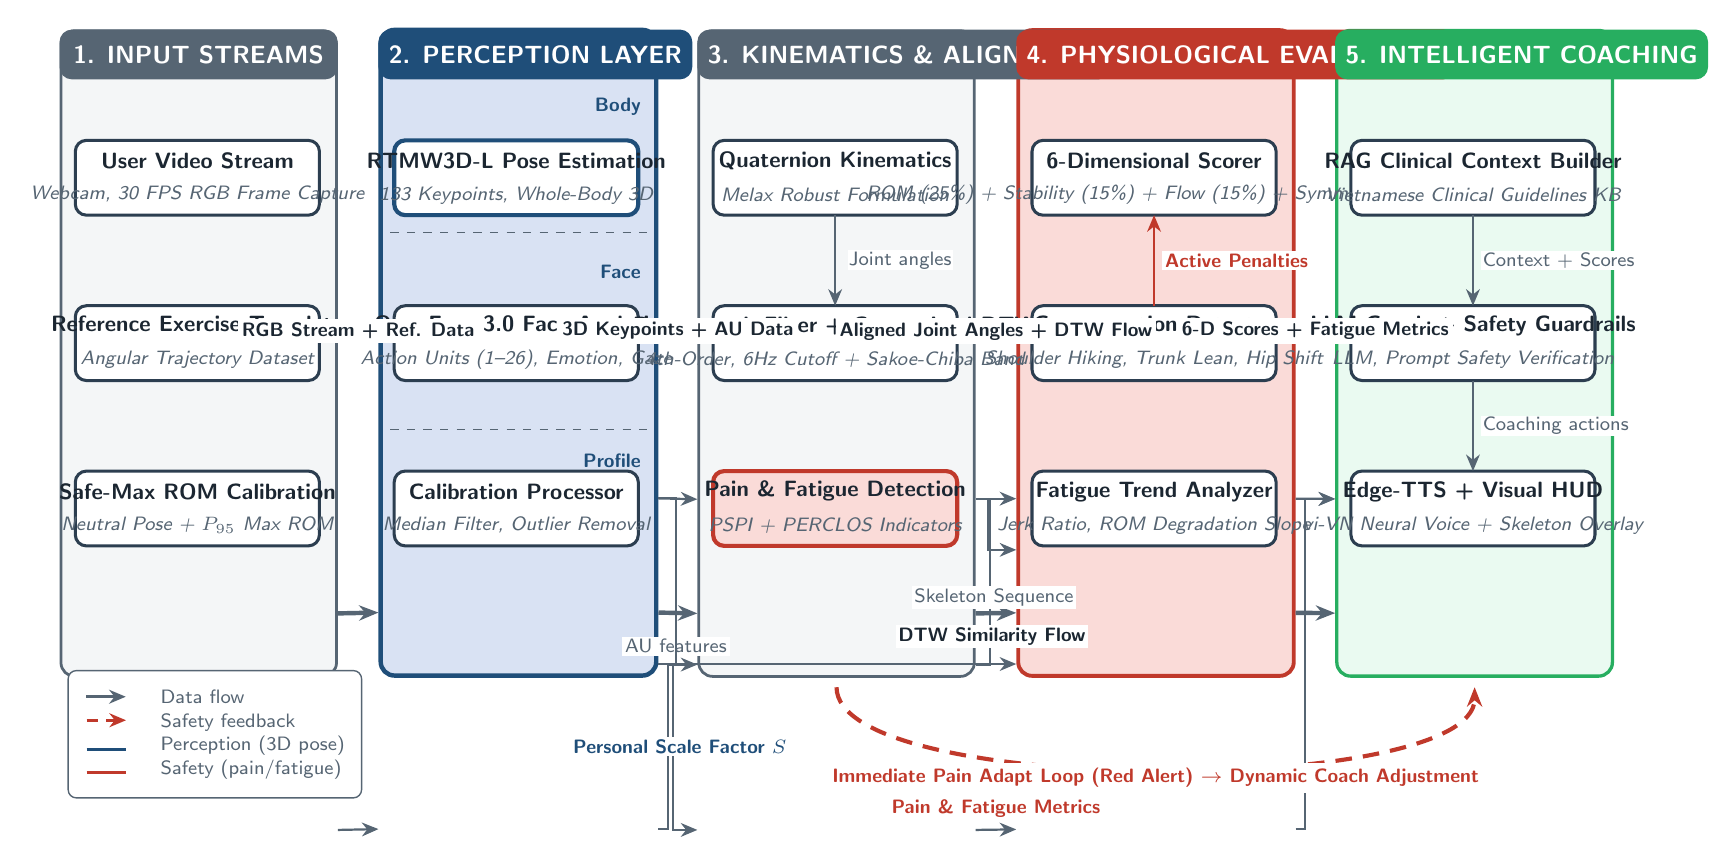
\begin{tikzpicture}[
    >={Stealth[length=6pt,width=5pt]},
    % Column background styles
    column/.style={
        rounded corners=5pt, draw=NeutralMid, line width=1pt,
        fill=NeutralColFill, minimum width=\colW cm, minimum height=\colH cm,
        inner sep=0pt, anchor=south west
    },
    perceptionColumn/.style={
        rounded corners=5pt, draw=AccentBlue, line width=1.6pt,
        fill=AccentBlueFill, minimum width=\colW cm, minimum height=\colH cm,
        inner sep=0pt, anchor=south west
    },
    evaluationColumn/.style={
        rounded corners=5pt, draw=AccentRed, line width=1.4pt,
        fill=AccentRedFill, minimum width=\colW cm, minimum height=\colH cm,
        inner sep=0pt, anchor=south west
    },
    outputColumn/.style={
        rounded corners=5pt, draw=OutputGreen, line width=1.2pt,
        fill=OutputGreenFill, minimum width=\colW cm, minimum height=\colH cm,
        inner sep=0pt, anchor=south west
    },
    % Title bar styles
    titleBar/.style={
        rounded corners=4pt, draw=AccentBlue, line width=0.9pt,
        fill=AccentBlue, minimum width=\colW cm, minimum height=\titleH cm,
        align=center, text=White, font=\bfseries\small, anchor=south west
    },
    titleBarEval/.style={
        rounded corners=4pt, draw=AccentRed, line width=0.9pt,
        fill=AccentRed, minimum width=\colW cm, minimum height=\titleH cm,
        align=center, text=White, font=\bfseries\small, anchor=south west
    },
    titleBarOutput/.style={
        rounded corners=4pt, draw=OutputGreen, line width=0.9pt,
        fill=OutputGreen, minimum width=\colW cm, minimum height=\titleH cm,
        align=center, text=White, font=\bfseries\small, anchor=south west
    },
    titleBarNeutral/.style={
        rounded corners=4pt, draw=NeutralMid, line width=0.9pt,
        fill=NeutralMid, minimum width=\colW cm, minimum height=\titleH cm,
        align=center, text=White, font=\bfseries\small, anchor=south west
    },
    % Edge label style
    edgeLabel/.style={
        font=\scriptsize\bfseries, text=TextMain, fill=White, inner sep=1.5pt
    },
    redEdgeLabel/.style={
        font=\scriptsize\bfseries\itshape, text=AccentRed, fill=White, inner sep=2pt
    },
  ]

  % ===========================================================================
  %  COLUMN COORDINATES (5 Columns) — pre-evaluated via \pgfmathsetmacro
  % ===========================================================================
  \pgfmathsetmacro{\xA}{0}
  \pgfmathsetmacro{\xB}{\colW+\colGap}
  \pgfmathsetmacro{\xC}{2*(\colW+\colGap)}
  \pgfmathsetmacro{\xD}{3*(\colW+\colGap)}
  \pgfmathsetmacro{\xE}{4*(\colW+\colGap)}
  \pgfmathsetmacro{\yTop}{0}
  \pgfmathsetmacro{\yBot}{-\colH}

  % ===========================================================================
  %  BACKGROUND COLUMNS (with color-coded semantics)
  % ===========================================================================
  % C1: Input — neutral gray
  \node[column]            (C1) at (\xA, \yBot) {};
  % C2: Perception — blue accent (core contribution: 3D pose)
  \node[perceptionColumn]  (C2) at (\xB, \yBot) {};
  % C3: Kinematics — neutral gray
  \node[column]            (C3) at (\xC, \yBot) {};
  % C4: Evaluation — red accent (safety contribution)
  \node[evaluationColumn]  (C4) at (\xD, \yBot) {};
  % C5: Coaching — green tint (output)
  \node[outputColumn]      (C5) at (\xE, \yBot) {};

  % ===========================================================================
  %  COLUMN HEADER TITLES
  % ===========================================================================
  \node[titleBarNeutral] (T1) at (\xA, \yTop-\titleH) {1. INPUT STREAMS};
  \node[titleBar]        (T2) at (\xB, \yTop-\titleH) {2. PERCEPTION LAYER};
  \node[titleBarNeutral] (T3) at (\xC, \yTop-\titleH) {3. KINEMATICS \& ALIGNMENT};
  \node[titleBarEval]    (T4) at (\xD, \yTop-\titleH) {4. PHYSIOLOGICAL EVALUATION};
  \node[titleBarOutput]  (T5) at (\xE, \yTop-\titleH) {5. INTELLIGENT COACHING};

  % ===========================================================================
  %  MODALITY DIVIDERS IN PERCEPTION COLUMN
  % ===========================================================================
  \draw[NeutralMid, line width=0.5pt, dash pattern=on 3pt off 3pt]
       ($(C2.north west)+(0.15,-2.6)$) -- ($(C2.north east)+(-0.15,-2.6)$);
  \draw[NeutralMid, line width=0.5pt, dash pattern=on 3pt off 3pt]
       ($(C2.north west)+(0.15,-5.1)$) -- ($(C2.north east)+(-0.15,-5.1)$);
  % Modality tags
  \node[font=\scriptsize\bfseries\itshape, text=AccentBlue, anchor=east]
       at ($(C2.north east)+(-0.1,-1.0)$) {Body};
  \node[font=\scriptsize\bfseries\itshape, text=AccentBlue, anchor=east]
       at ($(C2.north east)+(-0.1,-3.1)$) {Face};
  \node[font=\scriptsize\bfseries\itshape, text=AccentBlue, anchor=east]
       at ($(C2.north east)+(-0.1,-5.5)$) {Profile};

  % ===========================================================================
  %  STAGE 1: INPUT STREAMS (3 boxes)
  % ===========================================================================
  \compbox{\xA+\colW/2}{-1.85}
          {User Video Stream}
          {Webcam, 30 FPS RGB Frame Capture}

  \compbox{\xA+\colW/2}{-3.95}
          {Reference Exercise Template}
          {Angular Trajectory Dataset}

  \compbox{\xA+\colW/2}{-6.05}
          {Safe-Max ROM Calibration}
          {Neutral Pose + $P_{95}$ Max ROM}

  % ===========================================================================
  %  STAGE 2: PERCEPTION LAYER (3 boxes)
  % ===========================================================================
  \hlbox{\xB+\colW/2}{-1.85}
        {RTMW3D-L Pose Estimation}
        {133 Keypoints, Whole-Body 3D}

  \compbox{\xB+\colW/2}{-3.95}
          {OpenFace 3.0 Face Analysis}
          {Action Units (1--26), Emotion, Gaze}

  \compbox{\xB+\colW/2}{-6.05}
          {Calibration Processor}
          {Median Filter, Outlier Removal}

  % ===========================================================================
  %  STAGE 3: KINEMATICS & ALIGNMENT (3 boxes)
  % ===========================================================================
  \compbox{\xC+\colW/2}{-1.85}
          {Quaternion Kinematics}
          {Melax Robust Formulation}

  \compbox{\xC+\colW/2}{-3.95}
          {Butterworth Filter + Constrained DTW}
          {4th-Order, 6Hz Cutoff + Sakoe-Chiba Band}

  \redbox{\xC+\colW/2}{-6.05}
         {Pain \& Fatigue Detection}
         {PSPI + PERCLOS Indicators}

  % ===========================================================================
  %  STAGE 4: PHYSIOLOGICAL EVALUATION (3 boxes)
  % ===========================================================================
  \compbox{\xD+\colW/2}{-1.85}
          {6-Dimensional Scorer}
          {ROM (25\%) + Stability (15\%) + Flow (15\%) + Symmetry (15\%)}

  \compbox{\xD+\colW/2}{-3.95}
          {Compensation Detector}
          {Shoulder Hiking, Trunk Lean, Hip Shift}

  \compbox{\xD+\colW/2}{-6.05}
          {Fatigue Trend Analyzer}
          {Jerk Ratio, ROM Degradation Slope}

  % ===========================================================================
  %  STAGE 5: INTELLIGENT COACHING (3 boxes)
  % ===========================================================================
  \compbox{\xE+\colW/2}{-1.85}
          {RAG Clinical Context Builder}
          {Vietnamese Clinical Guidelines KB}

  \compbox{\xE+\colW/2}{-3.95}
          {LLM Coach + Safety Guardrails}
          {LLM, Prompt Safety Verification}

  \compbox{\xE+\colW/2}{-6.05}
          {Edge-TTS + Visual HUD}
          {vi-VN Neural Voice + Skeleton Overlay}

  % ===========================================================================
  %  PRIMARY INTER-COLUMN DATA FLOW ARROWS (thick, centered)
  % ===========================================================================
  \draw[NeutralMid, line width=1.6pt, -{Stealth[length=7pt,width=5.5pt]}]
       ($(C1.east)+(0,-3.3)$) -- ($(C2.west)+(0,-3.3)$);
  \draw[NeutralMid, line width=1.6pt, -{Stealth[length=7pt,width=5.5pt]}]
       ($(C2.east)+(0,-3.3)$) -- ($(C3.west)+(0,-3.3)$);
  \draw[NeutralMid, line width=1.6pt, -{Stealth[length=7pt,width=5.5pt]}]
       ($(C3.east)+(0,-3.3)$) -- ($(C4.west)+(0,-3.3)$);
  \draw[NeutralMid, line width=1.6pt, -{Stealth[length=7pt,width=5.5pt]}]
       ($(C4.east)+(0,-3.3)$) -- ($(C5.west)+(0,-3.3)$);

  % Primary flow labels
  \node[edgeLabel] at ($(C1.east)!0.5!(C2.west) + (0,0.28)$)
       {RGB Stream + Ref. Data};
  \node[edgeLabel] at ($(C2.east)!0.5!(C3.west) + (0,0.28)$)
       {3D Keypoints + AU Data};
  \node[edgeLabel] at ($(C3.east)!0.5!(C4.west) + (0,0.28)$)
       {Aligned Joint Angles + DTW Flow};
  \node[edgeLabel] at ($(C4.east)!0.5!(C5.west) + (0,0.28)$)
       {6-D Scores + Fatigue Metrics};

  % ===========================================================================
  %  INTERNAL MODULE-TO-MODULE ROUTING (thin arrows)
  % ===========================================================================

  % --- C1→C2 internal: ROM Calibration → Calibration Processor ---
  \draw[NeutralMid, line width=0.8pt, ->]
       ($(C1.east)+(0,-6.05)$) -- ($(C2.west)+(0,-6.05)$);

  % --- C2→C3 internal: RTMW3D → Quaternion Kinematics ---
  \draw[NeutralMid, line width=0.8pt, ->]
       ($(C2.east)+(0,-1.85)$) -- ($(C3.west)+(0,-1.85)$);

  % --- C2→C3 internal: OpenFace → Pain & Fatigue Detection ---
  \draw[NeutralMid, line width=0.8pt, ->]
       ($(C2.east)+(0,-3.95)$) -- +(0.18,0) |- ($(C3.west)+(0,-6.05)$);
  \node[font=\scriptsize, text=TextSub, fill=White, inner sep=1pt, anchor=south]
       at ($(C2.east)!0.45!(C3.west) + (0,-3.85)$) {AU features};

  % --- C2→C3 internal: Calibration Processor → DTW (Scale Factor S) ---
  \draw[NeutralMid, line width=0.8pt, ->]
       ($(C2.east)+(0,-6.05)$) -- +(0.12,0) |- ($(C3.west)+(0,-3.95)$);
  \node[font=\scriptsize\bfseries, text=AccentBlue, fill=White, inner sep=1pt]
       at ($(C2.east)!0.55!(C3.west) + (0,-5.0)$) {Personal Scale Factor $S$};

  % --- C3 internal: Quaternion → Butterworth/DTW (vertical) ---
  \draw[NeutralMid, line width=0.7pt, ->]
       ($(\xC+\colW/2,-1.85) + (0,-\boxH/2)$) --
       ($(\xC+\colW/2,-3.95) + (0,\boxH/2)$);
  \node[font=\scriptsize, text=TextSub, fill=White, inner sep=0.5pt, anchor=west]
       at ($(\xC+\colW/2+0.15,-2.9)$) {Joint angles};

  % --- C3→C4 internal: DTW → 6-D Scorer ---
  \draw[NeutralMid, line width=0.8pt, ->]
       ($(C3.east)+(0,-3.95)$) -- +(0.18,0) |- ($(C4.west)+(0,-1.85)$);
  \node[font=\scriptsize\bfseries, text=TextMain, fill=White, inner sep=1pt, anchor=south]
       at ($(C3.east)!0.4!(C4.west) + (0,-3.75)$) {DTW Similarity Flow};

  % --- C3→C4 internal: Butterworth → Scorer (symmetry/smoothness) ---
  \draw[NeutralMid, line width=0.7pt, ->]
       ($(C3.east)+(0,-1.85)$) -- +(0.15,0) |- ($(C4.west)+(0,-2.5)$);

  % --- C3→C4 internal: Pain & Fatigue → Fatigue Trend Analyzer ---
  \draw[NeutralMid, line width=0.8pt, ->]
       ($(C3.east)+(0,-6.05)$) -- ($(C4.west)+(0,-6.05)$);
  \node[font=\scriptsize\bfseries, text=AccentRed, fill=White, inner sep=1pt]
       at ($(C3.east)!0.5!(C4.west) + (0,-5.78)$) {Pain \& Fatigue Metrics};

  % --- C3→C4 internal: RTMW3D skeleton → Compensation Detector ---
  \draw[NeutralMid, line width=0.7pt, ->]
       ($(C2.east)+(0,-1.85)$) -- +(0.22,0) |- ($(C4.west)+(0,-3.95)$);
  \node[font=\scriptsize, text=TextSub, fill=White, inner sep=1pt]
       at ($(C3.east)!0.45!(C4.west) + (0,-3.1)$) {Skeleton Sequence};

  % --- C4 internal: Compensation → Scorer (active penalties) ---
  \draw[AccentRed, line width=0.8pt, ->]
       ($(\xD+\colW/2,-3.95) + (0,\boxH/2)$) --
       ($(\xD+\colW/2,-1.85) + (0,-\boxH/2)$);
  \node[font=\scriptsize\bfseries\itshape, text=AccentRed, fill=White, inner sep=1pt, anchor=west]
       at ($(\xD+\colW/2+0.1,-2.9)$) {Active Penalties};

  % --- C4→C5 internal: 6-D Scorer → RAG Context Builder ---
  \draw[NeutralMid, line width=0.8pt, ->]
       ($(C4.east)+(0,-1.85)$) -- ($(C5.west)+(0,-1.85)$);

  % --- C4→C5 internal: Fatigue Trends → RAG Context Builder ---
  \draw[NeutralMid, line width=0.8pt, ->]
       ($(C4.east)+(0,-6.05)$) -- +(0.12,0) |- ($(C5.west)+(0,-1.85)$);

  % --- C5 internal: RAG → LLM Coach ---
  \draw[NeutralMid, line width=0.7pt, ->]
       ($(\xE+\colW/2,-1.85) + (0,-\boxH/2)$) --
       ($(\xE+\colW/2,-3.95) + (0,\boxH/2)$);
  \node[font=\scriptsize, text=TextSub, fill=White, inner sep=0.5pt, anchor=west]
       at ($(\xE+\colW/2+0.1,-2.9)$) {Context + Scores};

  % --- C5 internal: LLM Coach → Edge-TTS + HUD ---
  \draw[NeutralMid, line width=0.7pt, ->]
       ($(\xE+\colW/2,-3.95) + (0,-\boxH/2)$) --
       ($(\xE+\colW/2,-6.05) + (0,\boxH/2)$);
  \node[font=\scriptsize, text=TextSub, fill=White, inner sep=0.5pt, anchor=west]
       at ($(\xE+\colW/2+0.1,-5.0)$) {Coaching actions};

  % ===========================================================================
  %  FEEDBACK LOOP: Pain & Fatigue → LLM Coach (red dashed Bezier arc)
  % ===========================================================================
  \coordinate (FBstart) at ($(C3.south)+(0,-0.12)$);
  \coordinate (FBend)   at ($(C5.south)+(0,-0.12)$);
  \draw[AccentRed, line width=1.5pt, dash pattern=on 6pt off 4pt,
        -{Stealth[length=7pt,width=5.5pt]}]
        (FBstart) .. controls +(0,-1.4) and +(0,-1.4) .. (FBend);
  \node[redEdgeLabel]
        at ($(FBstart)!0.5!(FBend)+(0,-1.15)$)
        {Immediate Pain Adapt Loop (Red Alert) $\rightarrow$ Dynamic Coach Adjustment};

  % ===========================================================================
  %  LEGEND (bottom-left)
  % ===========================================================================
  \node[rounded corners=3pt, draw=NeutralMid, line width=0.5pt,
        fill=White, inner sep=6pt, anchor=north west,
        font=\fontsize{7}{8.5}\selectfont, text=TextSub]
        (LG) at (\xA+0.1, \yBot+0.1) {%
        \begin{tabular}{@{}r l@{}}
        \tikz{\draw[NeutralMid, line width=1.2pt,->] (0,0) -- (0.5,0);} & Data flow \\
        \tikz{\draw[AccentRed, line width=1pt, dash pattern=on 4pt off 3pt,->] (0,0) -- (0.5,0);} & Safety feedback \\
        \tikz{\draw[AccentBlue, line width=1pt] (0,0) -- (0.5,0);} & Perception (3D pose) \\
        \tikz{\draw[AccentRed, line width=1pt] (0,0) -- (0.5,0);} & Safety (pain/fatigue) \\
        \end{tabular}%
        };

\end{tikzpicture}
\end{document}
